%%%%%%%%%%%%%%%%%%%%%%%%%%%%%%%%%%%%%%%%%%%%%%%%%%%%%%%%%%%%%%%%%%%%%%%%
% Plantilla TFG/TFM
% Escuela Politécnica Superior de la Universidad de Alicante
% Realizado por: Jose Manuel Requena Plens
% Contacto: info@jmrplens.com / Telegram:@jmrplens
%%%%%%%%%%%%%%%%%%%%%%%%%%%%%%%%%%%%%%%%%%%%%%%%%%%%%%%%%%%%%%%%%%%%%%%%

\chapter{Introduction}
\label{introduction}
In this first chapter we go over the main ideas of this work. In Section \ref{sec:overview} we will give an overview of the whole thesis. Section \ref{sec:motivation} will describe the motivations of this research. Finally, in Section \ref{sec:goals} we will point out the main proposal as well as the goals for this work.

\section{Overview}
\label{sec:overview}
In this bachelor's thesis we will be researching the Sim-2-Real field, specifically tackling the object detection problem from a semantic segmentation perspective. In the following chapters we will review and analyze the current state of art of some of the most important datasets, architectures and techniques used for semantic segmentation up to this day. We will also dive into the Sim-2-Real field, analyze some of the latest works as well as try to demonstrate how synthetic data can work in real-world domains.

This document is structured as follows: This first Chapter \ref{introduction} and Chapter \ref{marcoteorico} will go over the related works and State of Art of the Sim-2-Real and Semantic Segmentation field, as well as some works that served as inspiration while developing this project. Chapter \ref{metodologia} will describe the studied materials and methodologies used in this work. In Chapter \ref{desarrollo} we will describe the process of expansion of the UnrealROX framework as well as the Semantic Segmentation implementations. Finally, in Chapter \ref{conclusions} we go over the conclusions of this research.

\section{Motivation}
\label{sec:motivation}
The main motivation behind this project is to further investigate the Sim-2-Real and object detection field, specifically focusing on the UnrealROX project, and semantic segmentation techniques, concentrating our efforts in developing a user friendly framework for researches to easily generate synthetic data sequences in order to apply deep learning algorithms to real world environments.

This document was motivated by a collaboration with the \gls{dtic} and the \textit{3D Perception Lab} group, which mainly focuses on the fields of 3D Computer Vision, Machine Learning and \gls{gpu} Computing.

UnrealROX is a project directly correlated to \textit{The Robotrix: An eXtremely Photorealistic and Very-Large-Scale Indoor Dataset of Sequences with Robot Trajectories and Interactions} \cite{DBLP:journals/corr/abs-1901-06514} which was presented at the IROS conference in 2018. Funded by \textit{Ministerio de Economia y Competitividad} of the Spanish Government and directed by Jose Garcia-Rodriguez and Miguel Angel Cazorla-Quevedo, UnrealROX was the framework developed in order to generate said dataset.

\begin{figure}
	\centering
	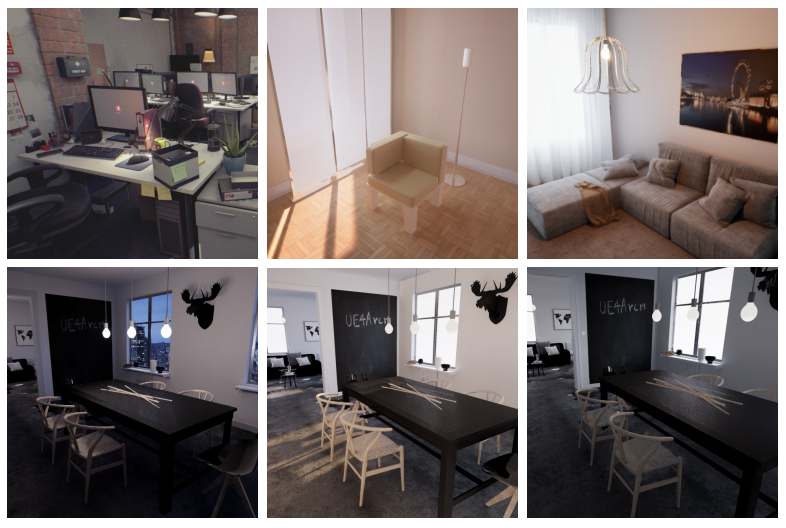
\includegraphics[width=0.7\linewidth]{archivos/robotrix}
		\caption{Snapshots of the Robotrix dataset extracted from \cite{DBLP:journals/corr/abs-1901-06514}.}
	\label{fig:robotrix}
\end{figure}

Synthetic data generation has been arising in popularity since the last few decades. Data driven algorithms have improved massively and good, quality datasets have been created in order to improve the accuracy of such algorithms. However it is still extremely expensive, both in time and resources, to create such datasets. This is where the Sim-2-Real field and the synthetic data generation comes into play, in this work we will specifically focusing on \textit{UnrealROX: An eXtremely Photorealistic Virtual Reality Environment for Robotics Simulations and Synthetic Data Generation} by \cite{DBLP:journals/corr/abs-1810-06936}.

\section{Proposal and Goals}
\label{sec:goals}
The main proposal for this work is to develop an extension to the UnrealROX project in order to automatize the synthetic data generation process, as well as conducting a study on how semantic segmentation architectures can transfer the knowledge of such synthetic data into the real-world domain.

As for the main objectives of this work, one of the first tasks was to establish a new type of \textit{Agent} in the framework that was not user-controlled, this would allow to generate data sequences without the need of a \gls{vr} Headset and user input, this 
provides a faster and more convenient way to obtain datasets.

The second main objective of this work was to test if such data would prove useful in real world problems. In order to demonstrate this, we will have to develop data driven algorithms and verify their accuracy with real-world datasets.

